\begin{requirement}
    As there shall be a support for data transformations between different schemas, the data transformations shall respect various ontology alignments to transform data between different ontologies. Alignments shall also be created during user modification of the ontology, between the modification and the original ontology.
    \label{requirement:ontology-alignments}
\end{requirement}

\textbf{Alignment} as defined in \cite{euzenat_ontology_2013} is a set of relations between entities \textit{usually} from different ontologies. These relations specify the semantic equivalence between the entities and create a mapping that can transform data from one ontology to another.

There are already well-known RDF predicates that can cover basic alignment. For semantically identical entities, we may use \verb|owl:equivalentClass| or \verb|skos:exactMatch|. A more useful RDF predicate is \verb|rdfs:subClassOf| for more specific classes representing things.

The latter is already used in the previous \autoref{requirement:inheritance}. Subclasses (i) reuse attributes and associations from their parent class but also semantically denote that (ii) the subclass can also be treated as "the parent class." The second point is an example of a simple ontology alignment.

\medskip

As an advanced example, suppose the address property that is used for delivery purposes. The address can be represented as one multi-line string value or as its parts such as street, number, etc. The most straightforward mapping would split the string by commas and new lines and join them back, respectively.

The user can then decide whether he/she wants to use the first or the second group of entities, and the transformation script would still be able to transform data between those two representations.

\begin{figure}[h!]\centering
  \centering
  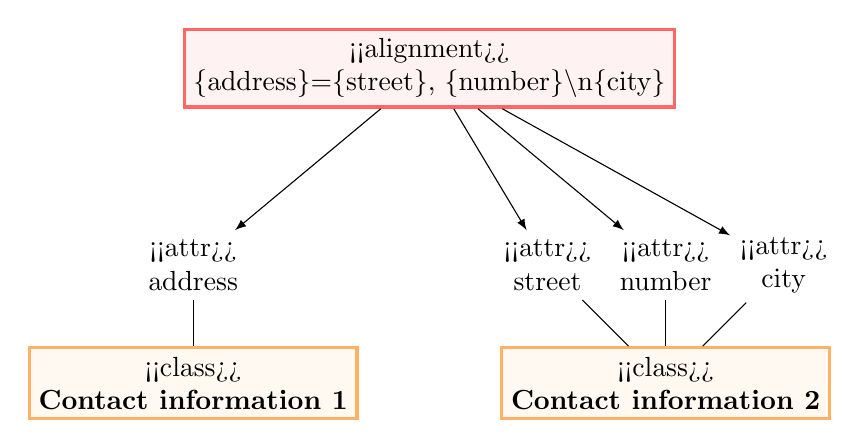
\begin{tikzpicture}[
    class/.style={shape=rectangle, draw=orange!60, fill=orange!5, very thick, minimum size=5mm,align=center},
    attribute/.style={align=center},
    mapping/.style={rectangle, draw=red!60, fill=red!5, very thick, minimum size=5mm},
  ]
    \node[class] (ci) at (0,0) {<<class>>\\\textbf{Contact information 1}};

    \node[class] (ci2) at (6,0) {<<class>>\\\textbf{Contact information 2}};

    \node[attribute] (a1) at (0,1.5) {<<attr>>\\address};
    \node[attribute] (a2) at (4.5,1.5) {<<attr>>\\street};
    \node[attribute] (a3) at (6,1.5) {<<attr>>\\number};
    \node[attribute] (a4) at (7.5,1.5) {<<attr>>\\city};

    \draw (ci) -- (a1);
    \draw (ci2) -- (a2);
    \draw (ci2) -- (a3);
    \draw (ci2) -- (a4);

    \node[mapping,align=center] (map) at (3,4) {<<alignment>>\\\{address\}=\{street\}, \{number\}\textbackslash n\{city\}};

    \draw[-latex] (map) -- (a1);
    \draw[-latex] (map) -- (a2);
    \draw[-latex] (map) -- (a3);
    \draw[-latex] (map) -- (a4);

  \end{tikzpicture}

  \caption{Example of mapping between different representations of address.}
\end{figure}

\medskip

The primary purpose of alignments is to use them for better data transformations, as different general schemas may use different parts of the ontology. By connecting them with alignment, we may be able to transform the data between a wider variety of schemas. We shall note that using multiple syntactically different ontologies in modeling is not our use case as our primary focus is to use ontology designed primarily for modeling. Nevertheless, there are some scenarios where some alignments are useful.

In general, we can use alignments directly from various ontologies (see \autoref{requirement:ontologies-on-the-web}) if the ontology supports it. As we have pointed out, we already use subclassing from the supported ontologies.

In addition to explicit use, alignments are also crucial for local modifications (see \autoref{requirement:pim-editing}). As we decide to introduce a new entity or modify others, it will be beneficial to keep the information that those entities are somehow related to the original ontology. Suppose the example with the address. We find that the address as a single field is not sufficient. Therefore, we split the address into individual parts and use them. The alignment together with the transformations still produces valid RDF data according to the original ontology.

This approach can even be used to create transformation scripts between old and new data if the ontology changes (see \autoref{requirement:evolution}). % We would simply instruct the propagation mechanism not to modify the PIM but rather create new entities and keep the old uninterpreted. We would then copy all schemas that were affected and evolute the copies. This would create new schemas and keeps old ones under the same PIM. Semantic mapping with data transformations would then generate the transformation scripts.

%We will keep the question behind the mapping open as it is way too advanced for the current state of the project. However, introducing a new PIM construct to the framework that maps the entities should not collide with the rest of the framework. And as it is at the PIM level, it would be possible to extract this information from CIM.